\section{Exclusive views}
\label{sec:directed}

%In this section, we will develop a consistent parameter estimate for a class of directed graphical models.
%The conditional moments $\mOpp{v}{i} \eqdef \Pr(x_v \mid h_i)$
%recovered from {\TensorFactorize}, are not the underlying parameters.
  %Once we recover the conditional moments $\mOpp{v}{j} \eqdef \Pr(x_v
  %| h_j)$ for some $v, j$, we present a systematic approach to learn the
  %conditional probability tables for every clique for a class of directed
  %graphical models.
In this section, we will use the conditional moments $\mOpp{v}{i} \eqdef
\Pr(x_v \mid h_i)$ recovered from the previous section
to compute the marginal distribution of sets of hidden variables $Z_S \eqdef \Pr(\bh_S)$,
taking us one step closer to the actual model parameters.
For clarity, we derive our algorithm in the infinite data limit,
although the actual algorithm works with estimates.

%%%%%%%%%%%%%%%%%%%%%%%%%%%%%%%%%%%%%%%%%%%%%%%%%%%%%%%%%%%%
\subsection{Example: directed grid model}
\label{sec:directedExample}

To gain some intuition, consider the directed grid model from \figureref{approach}.
%The model has eight observed variables $x^a_1, x^b_1 \cdots, x^a_4, x^b_4$ and four
  %hidden variables $h_1, \ldots, h_4$.
The parameters of this model are the conditional probability tables
$\pi \eqdef \Pr(h_1) \in \Re^k, T \eqdef \Pr(h_2 | h_1) = \Pr(h_3 | h_1) \in \Re^{k \times k},
V \eqdef \Pr(h_4 | h_2, h_3) \in \Re^{k \times k \times k}$ and $O \eqdef \Pr(x^a_i | h_i)
=  \Pr(x^b_i | h_i) \in \Re^{d \times k}$. 

\paragraph{Estimating $O$}
Since the observed variables $x^a_1, x^b_1, x^a_2$ are
  conditionally independent given $h_1$, we can $\TensorFactorize$ from
  \sectionref{setup} to recover $O$.

\paragraph{Estimating $\pi$}
The moments of $x^a_1$, $\mO_1 \eqdef \Pr(x^a_1)$ are directly related to
  $\pi$ by a linear system: $\mO_1 = O \pi$. 
If $O$ has full column rank, we can recover $\pi$ by taking the pseudoinverse: $\pi = O\pinv  \mO_1$.

\paragraph{Estimating $T$}
Similarly, we can write down the moments of $x^a_1, x^a_2$, $\mO_{12}
  \eqdef \Pr(x^a_1, x^a_2)$, in terms of the hidden marginals $\mH_{12}
  \eqdef \Pr(h_1, h_2)$ and solve for $\mH_{12}$:
\begin{align*}
\mO_{12} = O \mH_{12} O^\top \quad\Rightarrow\quad
  \mH_{12} = O\pinv  \mO_{12} O\pinvt .
\end{align*}
$T$ can be recovered from the $\mH_{12}$ by renormalizing the columns.

\paragraph{Estimating $V$}
Finally, we can estimate $V$ by renormalizing the hidden marginals
$\mH_{234} \eqdef \Pr(h_2, h_3, h_4)$ from the third-order moments
$\mO_{234} \eqdef \Pr(x^a_2, x^a_3, x^a_4)$:
\begin{align*}
  \mO_{234} = \mH_{234}(O, O, O) \quad\Rightarrow\quad
  \mH_{234} = \mO_{234}(O\pinv , O\pinv , O\pinv ).
\end{align*}

%%%%%%%%%%%%%%%%%%%%%%%%%%%%%%%%%%%%%%%%%%%%%%%%%%%%%%%%%%%%
\subsection{General algorithm}
\label{sec:directedGeneral}

  %Section~\ref{sec:directedGeneral} will describe the algorithm in full generality.
%For ease of exposition we make the following simplifications to our presentation:
%(i) we describe our algorithm entirely in the context of directed
  %graphical models, though it generalizes to undirected models;
%(iii) we present the algorithm solely in terms of linear algebraic operations;
  %\sectionref{piecewise} provides a statistically
  %more efficient estimator using composite likelihood.

The intuitions of the directed grid generalize readily to general graphs.
The key property required for our algorithm to work is as follows:
\begin{property}[Exclusive views]
  \label{prop:exclusive-views}
Given a graphical model $\sG$,
  a subset of hidden variables $S \subset \bh$ is said to satisfy the \emph{exclusive views property} if for
  each $h_i \in S$, the two conditions hold:
  (i) there exists some observed variable
  $x_{v}$ which is conditionally independent of the others $S \backslash \{ h_i \}$ given $h_i$,
  and (ii) the conditional moment matrix $\mOpp{v}{i} \eqdef
  \Pr(x_{v} \mid h_i)$ have full column rank $k$ and can be recovered.
We call $x_v$ an exclusive view of $h_i$ in $S$.
%If every hidden clique has the exclusive views property, then we say that $\sG$ does as well.
\end{property}

%%%%%%%%%%%%%%%%%%%%%%%%%%%%%%
\paragraph{Estimating hidden clique marginals}

We now show that if a subset of hidden variables $S$ has the exclusive views property,
then we can recover the marginal distribution $\Pr(\bh_S)$.
Consider any $S = \{i_1, \ldots, i_m\}$ with the exclusive views property. Let
  $x_{v_j}$ be an exclusive view for $h_{i_j}$ in $S$ and define $\sV
  = \{v_1, \ldots, v_m\}$. % be a set of exclusive views for the clique $S$.
By the exclusive views property,
the marginal over the observed variables $\Pr(\bx_\sV)$
factorizes according to the marginal over the hidden variables $\Pr(\bh_S)$
times the conditional moments:
\begin{align*}
  \mO_\sV 
  &\eqdef \Pr(\Sx{\sV}) \\
  &= \sum_{\vh_S} \Pr(\Sh{S}) 
                    \Pr(x_{v_1} | h_{i_1}) \cdots \Pr(x_{v_m} | h_{i_m}) \\
  &= Z_{S}(\mOpp{v_1}{i_1},\dots,\mOpp{v_m}{i_m}) \\
  &= Z_{S}(\mOppAll),
\end{align*}
where $\mOppAll = \mOpp{v_1}{i_1} \otimes \cdots \otimes \mOpp{v_m}{i_m}$ is the tensor product of
all the conditional moments.
Vectorizing, we have that
$Z_S \in \Re^{k^m}$,
$M_\sV \in \Re^{d^m}$,
and $\mOppAll \in \Re^{d^m \times k^m}$.
Since each $\mOpp{v}{i}$ has full column rank $k$,
$\mOppAll$ has full column rank $k^m$.
Succinctly, $\mO_\sV$ (which can be estimated directly from data)
is a linear function of $Z_S$ (what we seek to recover).
We can solve for the hidden marginals $Z_S$ simply by projecting $\mO_\sV$ onto the column
space of $\mOppAll$:
\begin{align*}
  Z_{S} &= \mO_\sV(\mOpp{v_1}{i_1}\pinv,\cdots,\mOpp{v_m}{i_m}\pinv).
\end{align*}

\algorithmref{learnclique} summarizes the procedure, \LearnClique.
Given $Z_S$, the conditional probability tables for $S$ can easily be
obtained via renormalization.
\begin{theorem}[Hidden marginals from exclusive views]
If $S \subseteq \bx$ is a subset of hidden variables with the exclusive views property,
then \algorithmref{learnclique} recovers the marginals $Z_S = \Pr(\bh_S)$.
\end{theorem}

%If each $\mOpp{v_j}{i_j}$ has full column rank, then

\begin{algorithm}
  \caption{\LearnClique~(pseudoinverse version)}
  \label{algo:learnclique}
  \begin{algorithmic}
    \REQUIRE Hidden subset $S$ with exclusive views (\propertyref{exclusive-views}).
    \ENSURE Marginal distribution $Z_S$.
      \STATE Identify exclusive views $\Sx{\sV} = \{x_{v_1}, \dots, x_{v_m}\}$.
      \STATE Return $\mH_S \gets \mO_{\sV}( \mOpp{v_1}{i_i}\pinv, \dots, {\mOpp{v_m}{i_m}}\pinv )$.
  \end{algorithmic}
\end{algorithm}

%%%%%%%%%%%%%%%%%%%%%%%%%%%%%%
\paragraph{Structural properties}

We have shown how to estimate the parameters of any clique that possesses the exclusive
  views property (\propertyref{exclusive-views}).
  But in a general graph, which cliques have this property?
  To provide intuition, we will provide more interpretable sufficient conditions
  and examples.

It is clear that having uniform bottlenecks implies part (ii)
of the exclusive views property (\propertyref{exclusive-views}) via \TensorFactorize,
but we will show that part (i) follows as well.

The exclusive views property 
Next, we define a (in analogy with biconnected component)
\begin{definition}[Bidependent set]
Given a graphical model $\sG$, we say that a subset of nodes $S$ is \emph{bidependent} if
conditioned on any $a \in S$, there is an active trail between any other two nodes $b,c \in S$.
\end{definition}
Intuitively
Note that all cliques are bidependent, but 
Bottlenecks provide three views, but to satisfy condition (ii) of \propertyref{exclusive-views},
only two is required.

Now we establish the link between bottlenecks and exclusive views:
\begin{lemma}[Uniformly bottlenecked implies exclusive views]
  \label{lem:bottleneck-views}  
% PL: simplify to cliques (this is also bad notation, since \sG is a set of cliques, not nodes)
%Let $\sG' = \{ h_{i_1}, \dots, h_{i_m} \} \subseteq \sG$ be
  %a connected subgraph of hidden variables.
  %If every hidden variable
  %$h_i \in \sG'$ is a bottleneck, then $\sG'$ has the exclusive views property.
  If a graphical model $\sG$ is faithful and uniformly bottlenecked, then
  every bidependent set in $\sG$ has the exclusive views property (and hence so does $\sG$).
\end{lemma}
\begin{proof}
We prove the contrapositive: suppose there exists a biconnected subgraph of $\sH \subset \sG$ consisting of hidden nodes
such that some $h_0 \in \sH$ does not have an exclusive view.
This means each observed variable $x_i$ in the graph is conditionally dependent on some
$h_i \in \sH \backslash \{h_0\}$ given $h_0$.
Consider any such two $x_1, x_2$.
Conditioned on $h_0$,
there is an active trail between $h_1$ and $h_2$ because $\sH$ is biconnected.
Thus, there is an active trail $x_1 - h_1 - h_2 - x_2$ conditioned on $h_0$.
Since $\sG$ is faithful, we have $x_1 \not\perp x_2 \mid h_0$.
As this holds for any $x_1,x_2$, $h_0$ cannot be a bottleneck.
\end{proof}

With this lemma in place, we present the full algorithm, $\LearnMarginals$,
in \algorithmref{directed}.

\begin{algorithm}
  \caption{\LearnMarginals}
  \label{algo:directed}
  \begin{algorithmic}
    \REQUIRE Graphical model $\sG$ satisfying \propertyref{bottleneck}, data $\sD$
    \ENSURE Marginals $Z_\sC$ for every clique $\sC \in \sG$

      \FOR{each hidden variable $h_i \in \bh$} 
        \STATE Apply $\TensorFactorize$ to learn conditional moments
        $\mOpp{v}{i}$ for every $v \in \sV_{h_i}$.

%    \COMMENT{Recover observation potentials $O$ using bottlenecks}
      \ENDFOR
%      \COMMENT{\textbf{Step 2:} Recover clique potentials from the piecewise likelihood.}
\FOR{every clique $\sC = \{h_{i_1}, \ldots, h_{i_m}\} \in \sG$} 
\STATE Apply $\LearnClique$ to learn the marginals $\mH_\sC$.
\ENDFOR
  \end{algorithmic}
\end{algorithm}


% DONE: move here because not central to story
\paragraph{Remarks.} We note that \propertyref{bottleneck} can be relaxed if some cliques
  share parameters.
For example, in the directed grid model, we can recover the conditional moments $O$ from
  $x^a_1, x^b_1$ and $x^a_2$ with $h_1$ as the bottleneck.
  Therefore, $h_2, h_3$ and $h_4$
  need not be bottlenecks, and we can omit the observations $x^b_2, x^b_3$ and $x^b_4$.

Our method also extends directly to case in which the observed variables
  are real-valued, while the hidden variables remain discrete. 
In this setting, the tensor factorization method of
  \citet{anandkumar13tensor} recovers the expected conditional means,
  $\mu_{vi} \eqdef \E(x_v | h_i) \in \Re^{d \times k}$ for each observed variable $x_v$ and
  hidden variable $h_i$.
\algorithmref{learnclique} and \algorithmref{directed} still apply and allow
  us to recover clique marginals $Z_\sC$.
%  \todo{make this a footnote if running out of space}
% PL: don't understand this comment
%In this case, we only require that the hidden variables in distinct
  %cliques share parameters.

\begin{figure}
  \centering
  \subfigure[Hidden Markov model] {
    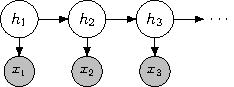
\includegraphics[width=0.45\columnwidth]{figures/hmm.pdf}
    \label{fig:examples-hmm}
  }
%  \subfigure[Directed grid model] {
%    \label{fig:examples-grid}
%    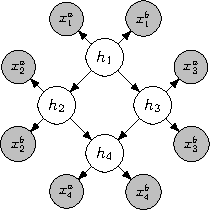
\includegraphics{figures/grid.pdf}
%  }
  \subfigure[Tree model] {
    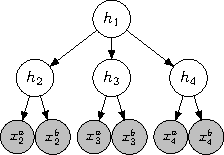
\includegraphics[width=0.45\columnwidth]{figures/tree.pdf}
    \label{fig:examples-tree}
  }
  \subfigure[Noisy-or model] {
    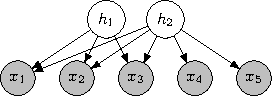
\includegraphics[height=5em]{figures/non-example.pdf}
    \label{fig:examples-noisy-or}
  }
  \caption{(a) and (b): graphs that satisfy the exclusive views property; (c) does not.}
  \label{fig:examples}
\end{figure}


\paragraph{Example: hidden Markov model.}

In the HMM (\figureref{examples-hmm}), the parameters
are $O \eqdef \Pr(x_i|h_i)$ and $T \eqdef \Pr(h_{i+1} | h_i)$
for all $i$.
While the first and last hidden variables $h_1, h_M$ in the
  sequence are not bottlenecks, they still have exclusive views ($x_1$ and
  $x_M$, respectively)
  due to parameter sharing.

\paragraph{Example: latent tree model.}

In the latent tree model (\figureref{examples-tree}), the parameters
are $\pi \eqdef \Pr(h_i)$, $T \eqdef \Pr(h_i | h_1)$ for $i \in \{2,3,4\}$,
and $O \eqdef \Pr(x^a_i | h_i) = \Pr(x^b_i | h_i)$ for $i \in \{2,3,4\}$.
Note that while $h_1$ is not directly connected to an observed variable,
  it is still a bottleneck, with views $x^a_2, x^a_3, x^a_4$.
We can recover $T$ from the clique $\{h_1, h_2\}$ by using views $x^a_2$
  (exclusive to $h_2$) and $x^a_3$ (exclusive to $h_1$).

\paragraph{Non-examples}
\label{sec:non-example}

There are certainly models which are identifiable but do not have exclusive views.
For example, \figureref{examples-noisy-or} shows
  a binary-valued noisy-or network which can be
  learned by the algorithm of \citet{halpern13noisyor},
  but does not satisfy the exclusive views property.
